\documentclass[11pt]{article}
\usepackage[utf8]{inputenc}
\usepackage[T1]{fontenc}
\usepackage{amsmath}
\usepackage{amssymb}
\usepackage{multicol}
\usepackage{geometry}
\usepackage{tikz}
\usepackage{enumitem}
\usepackage{xcolor}
\usepackage{titlesec}
\usetikzlibrary{shadows}
\usepackage{graphicx}
\usepackage{ragged2e}

% Layout
\geometry{a4paper, left=1cm, right=1cm, top=0.5cm, bottom=1.2cm}
\setlength{\columnseprule}{0.4pt}

% Estilo títulos
\titleformat{\section}{\normalfont\Large\bfseries\color{blue}}{\thesection}{1em}{}
\titleformat{\subsection}{\normalfont\large\bfseries\color{red}}{\thesubsection}{1em}{}

\title{\textcolor{blue}{Segunda Atividade: \\ Análise Combinatória}}
\author{Professor: Jefferson}
\date{}

\begin{document}

\maketitle
\vspace{-1cm}

\begin{center}
\large{Nome: \underline{\hspace{8cm}} \quad Turma: \underline{\hspace{3cm}}}
\end{center}

\begin{multicols}{2}

\section*{Exercícios}

\begin{enumerate}[leftmargin=*]

\item Uma urna contém 5 bolas vermelhas e 4 azuis. De quantas maneiras podemos retirar 3 bolas sem reposição?

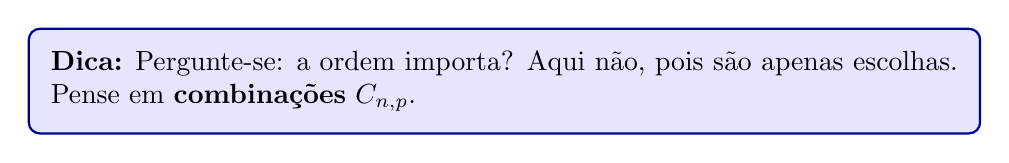
\begin{tikzpicture}
\node[rectangle, fill=blue!10, rounded corners, inner sep=8pt, draw=blue!60!black, thick, text width=0.95\linewidth, align=justify] {
\textbf{Dica:} Pergunte-se: a ordem importa? Aqui não, pois são apenas escolhas. Pense em \textbf{combinações} $C_{n,p}$.
};
\end{tikzpicture}

\vspace{5mm}

\item De quantas maneiras podemos organizar os alunos em uma fila de 7 lugares?

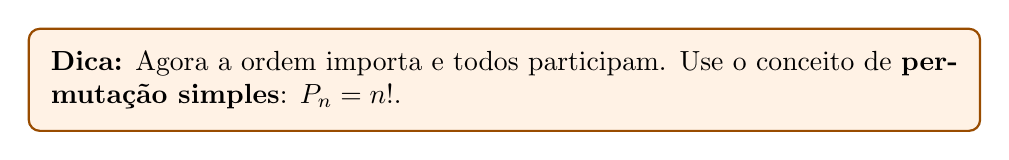
\begin{tikzpicture}
\node[rectangle, fill=orange!10, rounded corners, inner sep=8pt, draw=orange!60!black, thick, text width=0.95\linewidth, align=justify] {
\textbf{Dica:} Agora a ordem importa e todos participam. Use o conceito de \textbf{permutação simples}: $P_n = n!$.
};
\end{tikzpicture}

\vspace{5mm}

\item Quantos anagramas diferentes possui a palavra \textbf{SORRISO}?

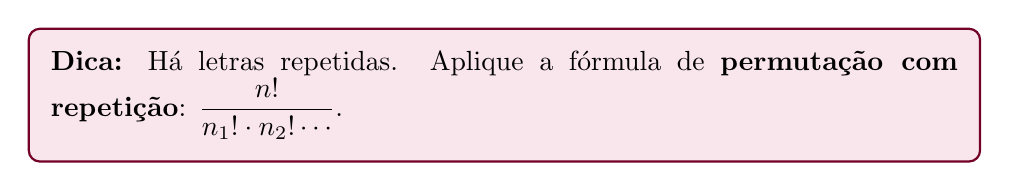
\begin{tikzpicture}
\node[rectangle, fill=purple!10, rounded corners, inner sep=8pt, draw=purple!60!black, thick, text width=0.95\linewidth, align=justify] {
\textbf{Dica:} Há letras repetidas. Aplique a fórmula de \textbf{permutação com repetição}: $\dfrac{n!}{n_1! \cdot n_2! \cdots}$.
};
\end{tikzpicture}

\vspace{5mm}

\item Um menu tem 6 pratos principais e 5 sobremesas. De quantas formas podemos escolher 1 prato e 1 sobremesa?

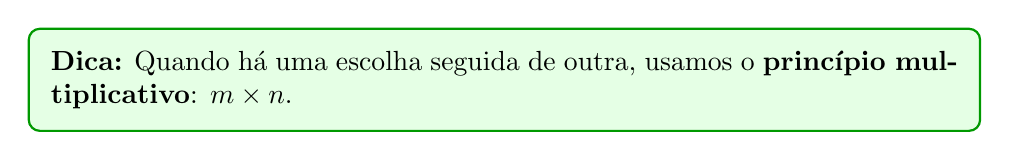
\begin{tikzpicture}
\node[rectangle, fill=green!10, rounded corners, inner sep=8pt, draw=green!60!black, thick, text width=0.95\linewidth, align=justify] {
\textbf{Dica:} Quando há uma escolha seguida de outra, usamos o \textbf{princípio multiplicativo}: $m \times n$.
};
\end{tikzpicture}

\vspace{5mm}

\item Em uma prova de múltipla escolha com 10 questões e 4 alternativas cada, de quantas maneiras um aluno pode marcar as respostas?

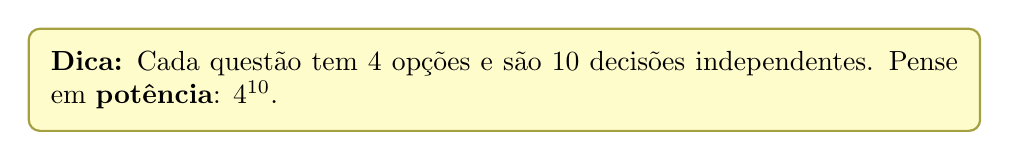
\begin{tikzpicture}
\node[rectangle, fill=yellow!20, rounded corners, inner sep=8pt, draw=yellow!60!black, thick, text width=0.95\linewidth, align=justify] {
\textbf{Dica:} Cada questão tem 4 opções e são 10 decisões independentes. Pense em \textbf{potência}: $4^{10}$.
};
\end{tikzpicture}

\vspace{5mm}

\item Quantas senhas de 3 dígitos distintos podem ser formadas usando os números de 0 a 9?

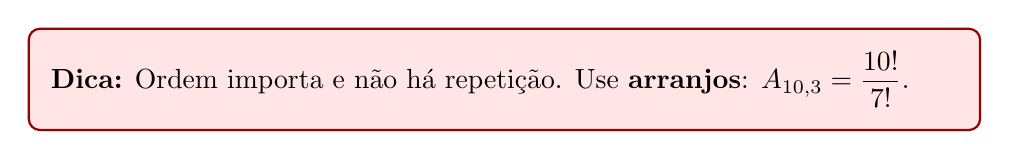
\begin{tikzpicture}
\node[rectangle, fill=red!10, rounded corners, inner sep=8pt, draw=red!60!black, thick, text width=0.95\linewidth, align=justify] {
\textbf{Dica:} Ordem importa e não há repetição. Use \textbf{arranjos}: $A_{10,3} = \dfrac{10!}{7!}$.
};
\end{tikzpicture}

\vspace{5mm}

\item Em uma sala com 12 alunos, quantos grupos de estudo de 4 pessoas diferentes podem ser formados?

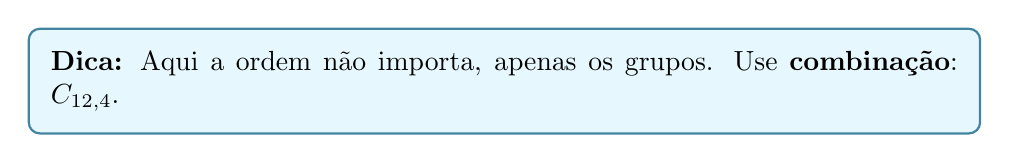
\begin{tikzpicture}
\node[rectangle, fill=cyan!10, rounded corners, inner sep=8pt, draw=cyan!60!black, thick, text width=0.95\linewidth, align=justify] {
\textbf{Dica:} Aqui a ordem não importa, apenas os grupos. Use \textbf{combinação}: $C_{12,4}$.
};
\end{tikzpicture}

\vspace{5mm}

\item Quantas placas de carro diferentes podem ser formadas com 3 letras (A–Z) seguidas de 4 números (0–9), permitindo repetições?

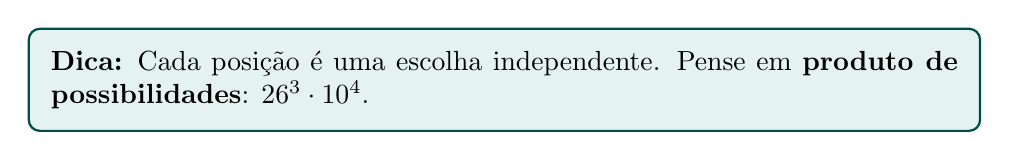
\begin{tikzpicture}
\node[rectangle, fill=teal!10, rounded corners, inner sep=8pt, draw=teal!60!black, thick, text width=0.95\linewidth, align=justify] {
\textbf{Dica:} Cada posição é uma escolha independente. Pense em \textbf{produto de possibilidades}: $26^3 \cdot 10^4$.
};
\end{tikzpicture}

\vspace{5mm}

\item Quantos subconjuntos com exatamente 3 elementos podem ser formados a partir de um conjunto com 9 elementos?

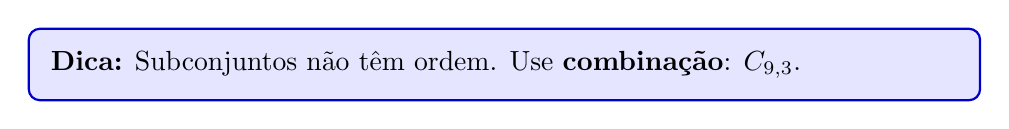
\begin{tikzpicture}
\node[rectangle, fill=blue!10, rounded corners, inner sep=8pt, draw=blue!80!black, thick, text width=0.95\linewidth, align=justify] {
\textbf{Dica:} Subconjuntos não têm ordem. Use \textbf{combinação}: $C_{9,3}$.
};
\end{tikzpicture}

\vspace{5mm}

\item Uma competição terá 1º, 2º e 3º lugar. Se há 15 competidores, de quantas maneiras diferentes os prêmios podem ser distribuídos?

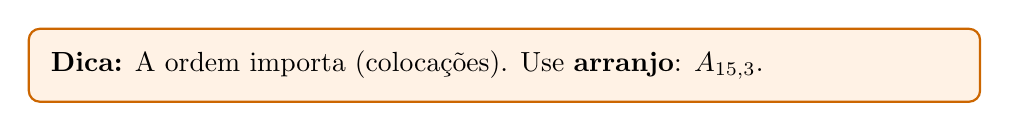
\begin{tikzpicture}
\node[rectangle, fill=orange!10, rounded corners, inner sep=8pt, draw=orange!80!black, thick, text width=0.95\linewidth, align=justify] {
\textbf{Dica:} A ordem importa (colocações). Use \textbf{arranjo}: $A_{15,3}$.
};
\end{tikzpicture}

\end{enumerate}

\begin{enumerate}[leftmargin=*, start=11]

\item Uma senha é formada por 2 letras seguidas de 3 números. Quantas senhas diferentes podem ser criadas permitindo repetição?

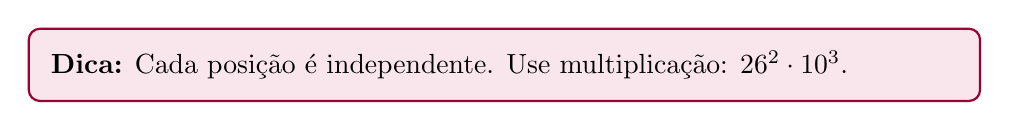
\begin{tikzpicture}
\node[rectangle, fill=purple!10, rounded corners, inner sep=8pt, draw=purple!80!black, thick, text width=0.95\linewidth, align=justify] {
\textbf{Dica:} Cada posição é independente. Use multiplicação: $26^2 \cdot 10^3$.
};
\end{tikzpicture}

\vspace{5mm}

\item Em uma estante há 8 livros diferentes. De quantas formas podemos escolher 5 para levar?

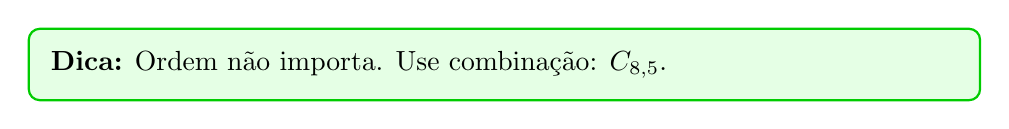
\begin{tikzpicture}
\node[rectangle, fill=green!10, rounded corners, inner sep=8pt, draw=green!80!black, thick, text width=0.95\linewidth, align=justify] {
\textbf{Dica:} Ordem não importa. Use combinação: $C_{8,5}$.
};
\end{tikzpicture}

\vspace{5mm}

\item Quantos números de 4 algarismos distintos podem ser formados usando os dígitos de 1 a 9?

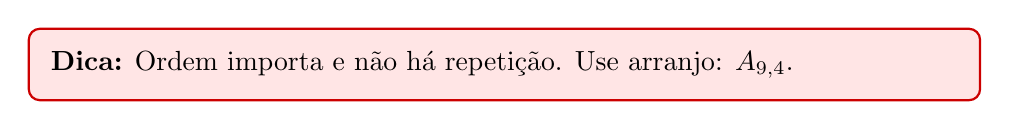
\begin{tikzpicture}
\node[rectangle, fill=red!10, rounded corners, inner sep=8pt, draw=red!80!black, thick, text width=0.95\linewidth, align=justify] {
\textbf{Dica:} Ordem importa e não há repetição. Use arranjo: $A_{9,4}$.
};
\end{tikzpicture}

\vspace{5mm}

\item De quantas formas podemos formar uma comissão de 2 homens e 3 mulheres a partir de 7 homens e 6 mulheres?

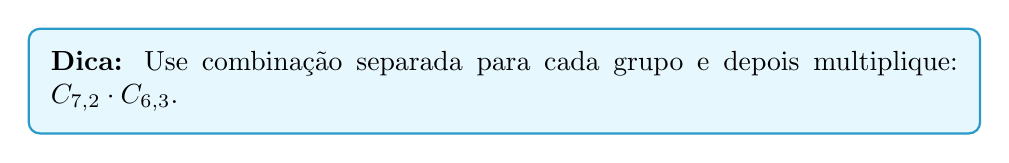
\begin{tikzpicture}
\node[rectangle, fill=cyan!10, rounded corners, inner sep=8pt, draw=cyan!80!black, thick, text width=0.95\linewidth, align=justify] {
\textbf{Dica:} Use combinação separada para cada grupo e depois multiplique: $C_{7,2} \cdot C_{6,3}$.
};
\end{tikzpicture}

\vspace{5mm}

\item Quantas formas diferentes existem para organizar 5 pessoas em uma mesa redonda?

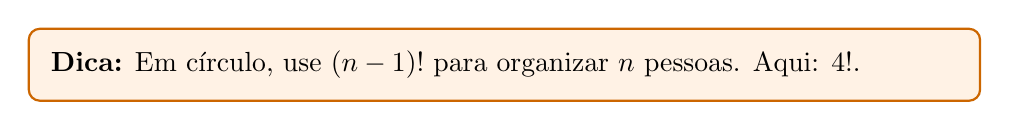
\begin{tikzpicture}
\node[rectangle, fill=orange!10, rounded corners, inner sep=8pt, draw=orange!80!black, thick, text width=0.95\linewidth, align=justify] {
\textbf{Dica:} Em círculo, use $(n-1)!$ para organizar $n$ pessoas. Aqui: $4!$.
};
\end{tikzpicture}

\vspace{5mm}

\item Quantos números de 3 algarismos podem ser formados se ao menos dois dígitos forem iguais?

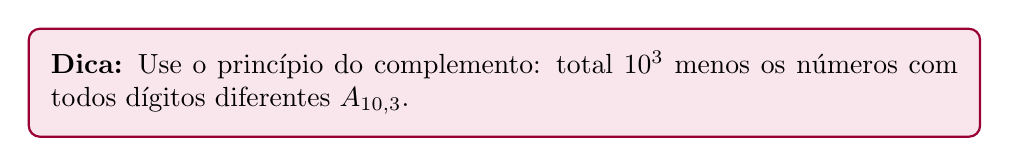
\begin{tikzpicture}
\node[rectangle, fill=purple!10, rounded corners, inner sep=8pt, draw=purple!80!black, thick, text width=0.95\linewidth, align=justify] {
\textbf{Dica:} Use o princípio do complemento: total $10^3$ menos os números com todos dígitos diferentes $A_{10,3}$.
};
\end{tikzpicture}

\vspace{5mm}

\item Quantos comitês de 4 pessoas diferentes podem ser formados em um grupo de 10 pessoas?

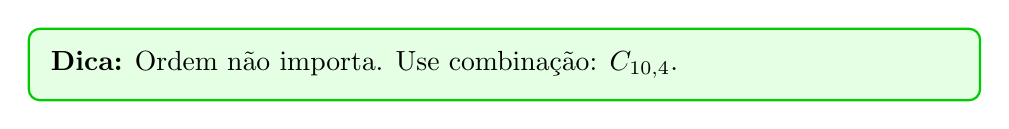
\begin{tikzpicture}
\node[rectangle, fill=green!10, rounded corners, inner sep=8pt, draw=green!80!black, thick, text width=0.95\linewidth, align=justify] {
\textbf{Dica:} Ordem não importa. Use combinação: $C_{10,4}$.
};
\end{tikzpicture}

\vspace{5mm}

\item Quantos anagramas diferentes podem ser feitos com a palavra \textbf{BANANA}?

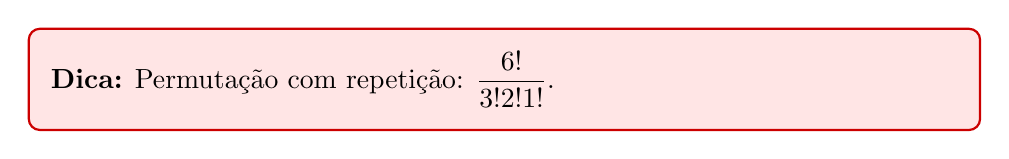
\begin{tikzpicture}
\node[rectangle, fill=red!10, rounded corners, inner sep=8pt, draw=red!80!black, thick, text width=0.95\linewidth, align=justify] {
\textbf{Dica:} Permutação com repetição: $\dfrac{6!}{3!2!1!}$.
};
\end{tikzpicture}

\vspace{5mm}

\item Uma escola deseja eleger um presidente, um vice e um secretário entre 12 alunos. De quantas formas é possível?

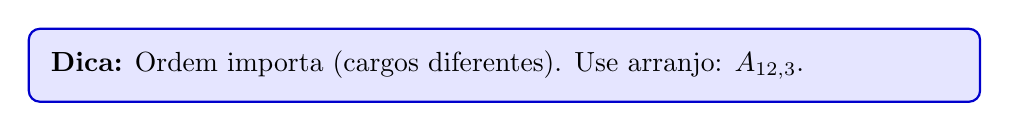
\begin{tikzpicture}
\node[rectangle, fill=blue!10, rounded corners, inner sep=8pt, draw=blue!80!black, thick, text width=0.95\linewidth, align=justify] {
\textbf{Dica:} Ordem importa (cargos diferentes). Use arranjo: $A_{12,3}$.
};
\end{tikzpicture}

\vspace{5mm}

\item Em um campeonato de 20 times, quantos jogos diferentes podem ser feitos se cada jogo envolve 2 times distintos?

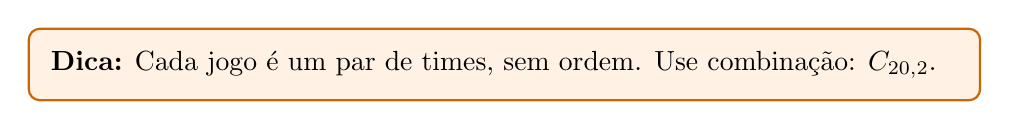
\begin{tikzpicture}
\node[rectangle, fill=orange!10, rounded corners, inner sep=8pt, draw=orange!80!black, thick, text width=0.95\linewidth, align=justify] {
\textbf{Dica:} Cada jogo é um par de times, sem ordem. Use combinação: $C_{20,2}$.
};
\end{tikzpicture}

\end{enumerate}


\end{multicols}
\end{document}

